\chapter{Módulo de gestión de proyectos y socias}

\bigskip

El módulo de gestión de proyectos y socias permite:

\liststyleLix
\begin{itemize}
\item Mantener la base social de vuestra organización.
\item Definir diferentes proyectos: talleres, cursos, proyectos de
cooperación, etc.
\item Asignar cuotas a las socias para generar remesas de recibos.
\item Generar ficheros de remesas para el procesamiento automatizado por
parte de bancos y cajas de ahorro.
\item Gestionar los pagos, impagos y devoluciones de los recibos.
\item Definir el formato de las partidas de gastos e ingresos para
presentar a la entidad financiadora.
\item Asignar los diferentes gastos e ingresos a las diferentes
partidas.


\bigskip
\end{itemize}
\section{Proyectos, socias y socios}
\appname considera a las personas socias de vuestra organización como
miembros de un determinado proyecto, en vez de presentar un apartado
específico para su gestión. Esta generalización permite tratar
todos los proyectos de la misma forma: añadir miembros, remesas,
recibos, cuotas, cuadros de financiación y de gastos, etc. \ Dentro
de la categoría de proyectos caben tanto talleres y jornadas a las
que es preciso inscribir miembros, como proyectos de cooperación con
entidades financiadoras, personal expatriado, cooperantes, etc. o
cualquier otro tipo de proyectos. En general, un proyecto es cualquier
acción de vuestra organización que está compuesta por personas,
que pueden tener o no una cuota por participar en ella y que tiene
asociada una partida de gastos e ingresos.

Desde este punto de vista, la base social de vuestra organización es
un proyecto más cuyos miembros son las personas socias.


\bigskip

\subsubsection{El fichero de proyectos}
Para añadir tanto vuestra base social como otro tipo de proyectos ve
al menú \textstyleGUIELEMENT{Asociación $\rightarrow $
Proyectos...} (ver \textit{Añadiendo algunos datos básicos},
página \pageref{ref:aadiendoalgunosdatosbasico}). Además de los
datos identificativos del proyecto, las fechas de alta y/o baja y el
estado, podrás añadir información para la posterior generación
de cuotas. Veamos algunos ejemplos de proyectos:

\paragraph{Base social de la organización}
Debes crear un proyecto para añadir a las personas socias de tu
organización cuyo nombre podría ser precisamente el de tu
organización. Una vez creado, selecciona la pestaña
\textstyleGUIELEMENT{M}\textstyleGUIELEMENT{iembros} y pulsa el botón
\textstyleGUIELEMENT{Añadir }para ir añadiendo socias. También
puedes importar los datos masivamente como se explica en el apartado
\textit{Importando masivamente datos de socias y socios} (página
\pageref{ref:Importandomasivamente}) del capítulo
\textbf{\textit{Poniendo en marcha \appname}}\textbf{\textit{.}} La
\textstyleGUIELEMENT{Fecha de inicio} del proyecto puede ser la de la
creación de vuestra organización, el \textstyleGUIELEMENT{Estado}
activo y la \textstyleGUIELEMENT{Fecha de fin} vacía. Si piensas
emitir recibos para el cobro de las cuotas, introduce el
\textstyleGUIELEMENT{Importe} y la \textstyleGUIELEMENT{Periodicidad de
la cuota} estándar. 

\paragraph{Proyecto de cooperación al desarrollo financiado por el
Ayuntamiento}
En estos proyectos, lo habitual es que la entidad financiadora requiera
una justificación de gastos Asociación $\rightarrow $e ingresos
según un formato establecido por ella estructurado en partidas. Como
cualquier otro proyecto, ve al menú \textstyleGUIELEMENT{Asociación
$\rightarrow $ Proyectos... }\textstyleGUIELEMENT{\textmd{\textup{y
rellena la información correspondiente. Activa la pestaña
}}}\textstyleGUIELEMENT{P}\textstyleGUIELEMENT{artidas}\textstyleGUIELEMENT{\textmd{\textup{
y añade las diferentes partidas de gastos e ingresos siguiendo la
estructura de la entidad financiadora. Lee el apartado
}}}\textstyleGUIELEMENT{\textmd{\textup{\ref{ref:Partidasproyectos}}}}\textstyleGUIELEMENT{\textmd{\textup{Partidas
de gastos e ingresos de
proyectos}}}\textstyleGUIELEMENT{\textmd{\textup{ para más
información.}}}

\paragraph[Jornadas]{\bfseries\itshape Jornadas}
Crea un proyecto con la \textstyleGUIELEMENT{Fecha de inicio} y
\textstyleGUIELEMENT{Fecha de fin} de las jornadas y pon el
\textstyleGUIELEMENT{Estado} activo. Si, como es habitual, el nombre de
las jornadas es largo, utiliza un nombre abreviado en el campo
\textstyleGUIELEMENT{Descripción} y el nombre completo en el campo
\textstyleGUIELEMENT{Descripción larga}. Si las jornadas son de pago,
introduce el \textstyleGUIELEMENT{Importe} y la
\textstyleGUIELEMENT{Periodicidad de la
cuota}\textstyleGUIELEMENT{\textmd{\textup{, que será
}}}\textstyleUserEntry{Puntual}\textstyleGUIELEMENT{\textmd{\textup{
caso de ser una sola cuota.}}}

\textstyleGUIELEMENT{\textmd{\textup{Ahora, activa la pestaña
}}}\textstyleGUIELEMENT{Miembros}\textstyleGUIELEMENT{\textmd{\textup{
y añade a las personas inscritas en las jornadas.}}}

\paragraph{Cursos}
Como en el caso de las jornadas, crea un proyecto con el nombre del
curso y añade los miembros al mismo. Si, por ejemplo, se trata de un
curso de pago de nueve meses en el que se paga mensualmente un importe
de \textstyleUserEntry{10{\texteuro}}, introduce en
\textstyleGUIELEMENT{Importe}, 10{\texteuro}, en
\textstyleGUIELEMENT{Periodicidad de la cuota},
\textstyleUserEntry{MENSUAL}\textstyleGUIELEMENT{ }y en
\textstyleGUIELEMENT{Número de cuotas}, \textstyleUserEntry{9.}

\subsubsection{El fichero de miembros de proyectos}
En este fichero se define el tipo de afiliación de cada socia a cada
proyecto, es decir, el tipo de socia, el estado: activo o inactivo, las
fechas de alta y de baja, la cuota y la forma de pago y cuenta
bancaria, en su caso, para el cobro de las cuotas.

Mediante el tipo de socia y la forma de pago se puede gestionar todas
las variedades de pagos de recibos que se pueden presentar en la
asociación. Lee el apartado \ref{ref:Remesasyrecibos} Remesas y
recibos para más información.

\section{Remesas y recibos}
\label{ref:Remesasyrecibos}\appname permite un control fiel de los
cobros de las cuotas de cualquier proyecto, ya sean las cuotas
periódicas de nuestra organización o las cuotas puntuales de una
jornada o las cuotas mensuales de un curso anual. \ Toda esta variedad
de cuotas se define mediante información general del proyecto e
información particular de cada miembro.

\subsubsection{Definición de las cuotas de los proyectos}
Al crear un proyecto, se define el importe y periodicidad de las cuotas
estándar. Veamos algunos ejemplos:

\paragraph{Base social de la organización}
Si tu organización solicita a sus miembros el pago de una cuota anual
de 60{\texteuro}, definiríamos el valor de
\textstyleGUIELEMENT{Importe} a \textstyleUserEntry{60} y el de
\textstyleGUIELEMENT{Periodicidad de la cuota} a
\textstyleUserEntry{anual}. El \textstyleGUIELEMENT{Número de cuotas}
quedaría a cero puesto que no hemos definido una fecha de fin para el
proyecto. 

Los casos particulares a la hora de pagar la cuota, como cuotas
reducidas o formas de pago aplazadas o en distintas entregas, se
definirían posteriormente en la ficha de cada miembro del proyecto.

\paragraph[Curso]{Curso}
Imagina un curso de nueve meses impartido por vuestra organización por
un importe total de 900{\texteuro}. Si quieres generar los recibos del
curso cada mes, \ define el valor de \textstyleGUIELEMENT{Importe} a
\textstyleUserEntry{90}, el de \textstyleGUIELEMENT{Periodicidad de la
cuota} a\textstyleUserEntry{ mensual} y el
\textstyleGUIELEMENT{Número de cuotas }a \textstyleUserEntry{9}. Si
los quieres generar cada trimestre, haz \textstyleGUIELEMENT{Importe} =
\textstyleUserEntry{270}, \textstyleGUIELEMENT{Periodicidad de la
cuota} =\textstyleUserEntry{ trimestral} y
\textstyleGUIELEMENT{Número de cuotas =} \textstyleUserEntry{3}. Si
los quieres anuales, haz \textstyleGUIELEMENT{Importe} =
\textstyleUserEntry{900}, \textstyleGUIELEMENT{Periodicidad de la
cuota} =\textstyleUserEntry{ anual} y \textstyleGUIELEMENT{Número de
cuotas =} 1.

\paragraph{Taller de fin de semana}
En este caso, quieres cobrar una sola cuota de inscripción al taller
de 10{\texteuro}. Haz \textstyleGUIELEMENT{Importe} =
1\textstyleUserEntry{0}, \textstyleGUIELEMENT{Periodicidad de la cuota}
=\textstyleUserEntry{ puntual }y \textstyleGUIELEMENT{Número de
cuotas =} 1.


\bigskip

\subsubsection{Definición de la forma de pago de cada socia}
En el apartado anterior has definido el importe, número y periodicidad
de las cuotas estándar de cada proyecto. Pero cada miembro puede
decidir pagar las cuotas de forma distinta, además de poder acogerse
a reducciones del importe de la cuota por diferentes motivos. Estos
casos particulares se definen utilizando los ficheros de Tipos de socia
y de Formas de pago.

\paragraph{El fichero de tipos de socia}
Para cada miembro es obligatorio definir un tipo de socia que permite,
aparte de clasificarlos, definir el porcentaje sobre la cuota total del
proyecto que deben pagar. Por ejemplo, si la gente desempleada paga
solo el 50\% de la cuota, crea un nuevo tipo de socia desde el menú
\textstyleGUIELEMENT{Asociación $\rightarrow $ Tipos de socia... }al
que puedes llamar \textstyleUserEntry{Personas desempleadas} y en el
campo \textstyleGUIELEMENT{\% cuota} introduce un
\textstyleUserEntry{50}. Ten en cuenta que el campo
\textstyleGUIELEMENT{\% cuota} se refiere al porcentaje que se paga, no
a la reducción. Así, si un tipo de socia tiene una reducción del
30\% del importe de la cuota, debes introducir un 70\%.

\paragraph{El fichero de formas de pago}
Hasta ahora has definido el importe de las cuotas y su periodicidad
según está definido en tu organización. Pero es probable que las
socias decidan pagar las cuotas con una periodicidad menor a la que has
definido. Para ello puedes crear distintas formas de pago desde el
menú \ \textstyleGUIELEMENT{Contabilidad$\rightarrow $ Formas de
pago... }donde puedes definir el número de plazos y el intervalo de
días entre ellos.

Es obligatorio definir una forma de pago para cada miembro. La forma
más habitual será la del que paga las cuotas en un solo plazo
cuando se le presentan. Para ello, define una forma de pago con el
valor \textstyleUserEntry{1} en el campo \textstyleGUIELEMENT{Número
de plazos}.

Para permitir a las socias pagar una cuota anual de forma semestral,
basta con definir la periodicidad de la cuota en el proyecto a anual y
una forma de pago para la socia que incluya dos plazos.

\subsubsection{Emisión de remesas de recibos}
Una vez definidos todos los datos anteriores: Importe, número y
periodicidad de las cuotas en el proyecto, porcentaje de cuota a
aplicar a la socia y forma de pago, puedes generar una remesa de
recibos. 

Por diseño, todos los recibos en \appname deben pertenecer a una
remesa, aunque ésta contenga un solo recibo. Por lo tanto, crea una
nueva remesa desde la pestaña
\textstyleGUIELEMENT{R}\textstyleGUIELEMENT{emesas} que aparece cuando
entras a modificar un proyecto. También puedes hacerlo desde
\textstyleGUIELEMENT{Asociación }\textstyleGUIELEMENT{$\rightarrow
$}\textstyleGUIELEMENT{ Proyectos ...}.

Introduce los datos para identificar la remesa: el proyecto a la que
pertenece, el número, la descripción y las fechas de emisión y de
cargo de los recibos. Si esta remesa va a ser enviada a una caja de
ahorros o banco para su cobro, introduce el código de la cuenta
bancaria donde queréis que sean ingresados los importes de los
recibos.

Una vez guardada la remesa, puedes añadir recibos de dos maneras:
manual y automáticamente. Aunque vas a utilizar casi siempre la forma
automática, comenzaremos explicando la forma manual para que te
familiarices con los recibos y porque en alguna ocasión necesitarás
añadir un sólo recibo.

\paragraph{Añadiendo recibos manualmente}
Entra en \textstyleGUIELEMENT{Asociación
}\textstyleGUIELEMENT{$\rightarrow $}\textstyleGUIELEMENT{ Proyectos
... }y modifica el proyecto y pulsa en la pestaña
\textstyleGUIELEMENT{R}\textstyleGUIELEMENT{emesas} y modifica la
remesa a la que quieres añadir los recibos. Pulsa el botón
\textstyleGUIELEMENT{Añadir recibo}.

\begin{center}
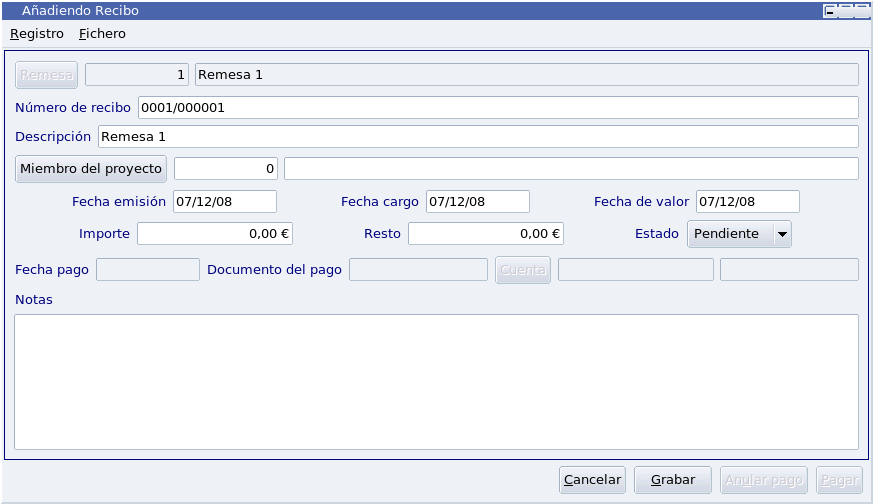
\includegraphics[width=11.956cm,height=7.419cm]{manual-img20.png}
\captionof{figure}[Dando de alta un recibo]{Dando de alta un recibo}

\end{center}
En principio, el número y la descripción del recibo, así como las
fechas de emisión, cargo y valor, \ aparecen automáticamente,
aunque puedes cambiarlas.

Elige el miembro e introduce el importe y resto del recibo. 

La fecha de valor es útil para saber a qué periodo de emisión
pertenece el recibo para evitar emitir recibos duplicados.

\paragraph{Generando remesas automáticamente}
\appname permite generar remesas con los recibos de todos o una parte de
los miembros un proyecto mediante la opción del menú
\textstyleGUIELEMENT{Asociación }\textstyleGUIELEMENT{$\rightarrow
$}\textstyleGUIELEMENT{ Generar recibos ...}

\begin{center}
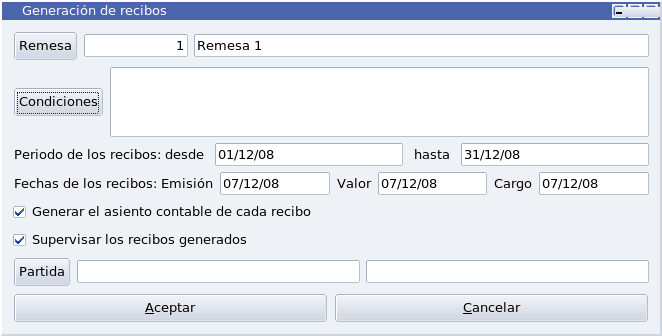
\includegraphics[width=10.261cm,height=5.041cm]{manual-img21.png}
\captionof{figure}[Generando recibos automáticamente]{Generando
recibos automáticamente}

\end{center}
Elige la remesa que contendrá los recibos y, si quieres seleccionar
una parte de los miembros del proyecto, hazlo pulsando el botón
\textstyleGUIELEMENT{Condiciones}. \ Si no, se generarán recibos para
todos los miembros. Introduce el período para el cual se generarán
los recibos y las fechas de emisión, valor y cargo de los mismos. 

Si quieres generar los asientos contables correspondientes a los
recibos, marca la casilla \textstyleGUIELEMENT{Generar
}\textstyleGUIELEMENT{el asiento contable de cada recibo}. Si además,
quieres que los asientos se asignen a una determinada partida de
ingresos del proyecto, elígela. Por último, si quieres revisar los
recibos generados uno por uno antes de que se graben, marca la casilla
\textstyleGUIELEMENT{Revisar los recibos generados}. 

\subsubsection{Envío de remesas a la entidad financiera}
Entra en \textstyleGUIELEMENT{Asociación
}\textstyleGUIELEMENT{$\rightarrow $}\textstyleGUIELEMENT{ Proyectos
... }y modifica el proyecto y pulsa en la pestaña
\textstyleGUIELEMENT{R}\textstyleGUIELEMENT{emesas} y selecciona la
remesa del proyecto que quieres enviar a la entidad financiera para el
tratamiento informatizado de los cobros.

Asegúrate de que has introducido el código de cuenta de abono de tu
caja de ahorros o banco. Revisa también que has introducido el
código de la cuenta bancaria de cada miembro al que quieres cargarle
el recibo. Pulsa el botón \textstyleGUIELEMENT{Generar CB19}. 

Aparecerá una ventana para que introduzcas el nombre y el lugar donde
se va a guardar el \ fichero que has de enviar a la entidad bancaria.
Una vez finalizado el proceso, un mensaje te indicará cuántos
recibos se han generado y cuántos no por diversos motivos: miembro no
activo, númeo de cuenta vacío, etc.

\subsubsection{Gestión de los pagos de los recibos}
Desde el fichero de recibos, ya sea directamente desde
\textstyleGUIELEMENT{Asociación }\textstyleGUIELEMENT{$\rightarrow
$}\textstyleGUIELEMENT{ Recibos ... }o desde\textstyleGUIELEMENT{
Asociación }\textstyleGUIELEMENT{$\rightarrow $}\textstyleGUIELEMENT{
Proyectos }\textstyleGUIELEMENT{$\rightarrow $}\textstyleGUIELEMENT{
Remesas }\textstyleGUIELEMENT{$\rightarrow $}\textstyleGUIELEMENT{
Recibos, }se pueden realizar o anular los pagos. Para realizar el pago
de un recibo pendiente, selecciónalo y pulsa el botón Pagar. A
continuación, introduce la fecha, el importe, el documento y la
cuenta del pago. En estas circunstancias, pueden darse tres casos:

\liststyleLx
\begin{enumerate}
\item El importe introducido coincide con el resto del recibo. El recibo
cambia del estado pendiente al estado pagado y se genera el
correspondiente asiento en contabilidad.
\item El importe introducido es menor que el resto del recibo. El recibo
original queda pagado por la cantidad introducida y se genera un nuevo
recibo con el nuevo resto. Se genera automáticamente el asiento del
pago.
\item El importe introducido es mayor que el resto del recibo. El recibo
original se paga y mientras el importe introducido sea mayor, se eligen
recibos de la misma persona (aunque pueden ser de otros proyectos y/o
remesas) para ir descontando su importe. Al final, se genera un asiento
que recoge todos los pagos conjuntos.
\end{enumerate}

\bigskip

\subsubsection{Impresión del recibí}
Sobre cualquier recibo pagado se puede pulsar CTRL+P para obtener un
informe equivalente a un recibí. El informe se llama recibi.rtk y se
puede personalizar.


\bigskip


\bigskip


\bigskip


\bigskip


\bigskip

\clearpage
\bigskip

\section{Partidas de gastos e ingresos de proyectos}
\label{ref:Partidasproyectos}\label{ref:Partidasproyetos}Para los
proyectos en los que es necesario presentar una justificación de
gastos e ingresos a la entidad financiadora, se pueden definir las
partidas en la pestaña
\textstyleGUIELEMENT{P}\textstyleGUIELEMENT{artidas} del fichero de
proyectos. Para el resto de proyectos, es suficiente con la
contabilidad, aunque también se pueden crear partidas.

Ve al menú \textstyleGUIELEMENT{Asociación
}\textstyleGUIELEMENT{$\rightarrow $}\textstyleGUIELEMENT{ Proyectos
...} y crea o modifica un proyecto. Verás que hay cuatro solapas,
pulsa sobre la última
(\textstyleGUIELEMENT{P}\textstyleGUIELEMENT{artidas}) y verás la
plantilla vacía. Pulsa el botón \textstyleGUIELEMENT{Añadir
partida} y rellena los datos.

Los códigos y las descripciones son totalmente libres aunque no pueden
estar repetidos dentro de un mismo proyecto. Las partidas se pueden
organizar jerárquicamente utilizando el campo
\textstyleGUIELEMENT{Código de la partida madre}, de modo que los
importes que se adjudiquen a esta partida se sumen también a su
partida madre. El \textstyleGUIELEMENT{Tipo }puede ser G para gastos, I
para ingresos y T para el total (Ingresos -- Gastos). El
\textstyleGUIELEMENT{Presupuesto} es útil para compararlo con el
\textstyleGUIELEMENT{Importe} final. Graba la partida y continúa
rellenando la plantilla completamente.

\begin{center}
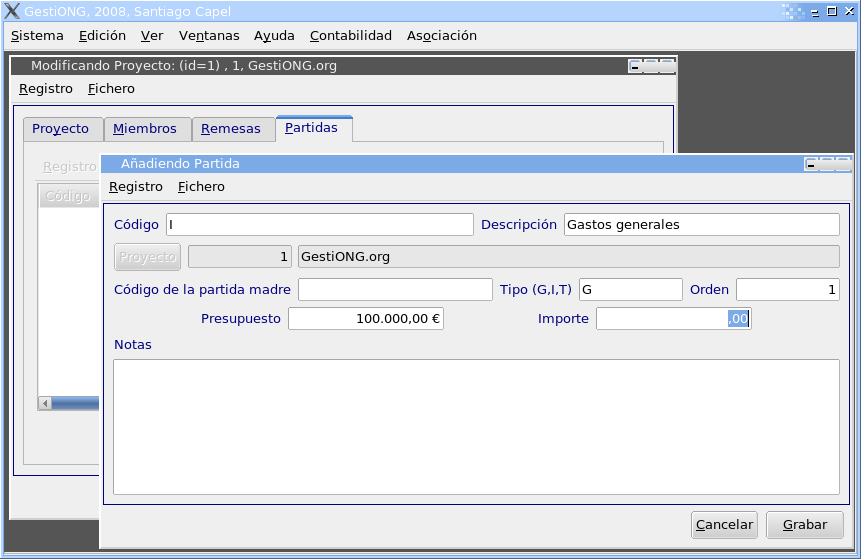
\includegraphics[width=9.738cm,height=6.452cm]{manual-img22.png}
\captionof{figure}[Dando de alta una partida]{Dando de alta una partida}

\end{center}
Se pueden actualizar estas partidas de forma manual para introducir los
gastos e ingresos de cada proyecto y luego realizar un informe para
presentarlo a nuestra financiadora. Sin embargo, lo más fácil es
utilizar el módulo de contabilidad para introducir los movimientos
económicos y asociarlos a partidas de nuestro proyecto, como se
explica en el apartado Asignando apuntes a partidas del capítulo V,
Módulo de contabilidad.

\chapter{Módulo socias}

\subsection{Añadiendo algunos datos básicos}
\label{ref:aadiendoalgunosdatosbasico}El elemento fundamental de
\appname es el proyecto. Un proyecto contiene miembros, tiene una
duración determinada y permite un control económico de gastos e
ingresos. De hecho, todos los socios y socias de tu organización
deberán estar incluidos en un proyecto. Vas a crear este primer
proyecto.

Selecciona el menú \textstyleGUIELEMENT{Asociación $\rightarrow $
Proyectos}, y pulsa el botón \textstyleGUIELEMENT{Añadir}
(\textstyleGUIELEMENT{o Ctrl+A}) en la ventana que aparece. El
\textstyleGUIELEMENT{Código} debería ser el
{\textquotesingle}\textit{1{\textquotesingle}}, tal y como aparece en
la \figurename~\ref{seq:refIllustration6}, la descripción podría
ser {\textquotesingle}\textit{Socios y socias de nuestra
asociación}{\textquotesingle}, la \textstyleGUIELEMENT{Fecha de alta}
la que corresponda y el \textstyleGUIELEMENT{Estado}
{\textquotesingle}\textit{Activo{\textquotesingle}}. Una vez
introducidos todos los datos, pulsa el botón
\textstyleGUIELEMENT{Grabar}.

\begin{center}
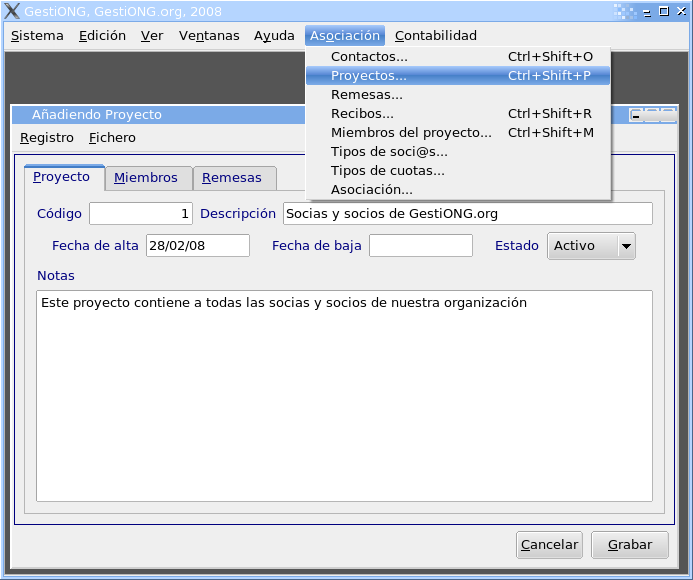
\includegraphics[width=9.618cm,height=6.354cm]{manual-img11.png}
\captionof{figure}[Añadiendo el proyecto principal]{Añadiendo el
proyecto principal}
\label{seq:refIllustration6}

\end{center}
Ahora selecciona el menú \textstyleGUIELEMENT{Asociación
$\rightarrow $ Tipos de
}\href{mailto:soci@s}{\textstyleGUIELEMENT{soci@s}} y añade un tipo
de socia (pulsa \textstyleGUIELEMENT{Ctrl+A}) con
\textstyleGUIELEMENT{Código}
{\textquotesingle}\textit{1}{\textquotesingle} y
\textstyleGUIELEMENT{Descripción}
{\textquotesingle}\textit{Normal}{\textquotesingle}. Selecciona
\textstyleGUIELEMENT{Asociación $\rightarrow $ Tipos de cuotas} y
añade un tipo de cuota con \textstyleGUIELEMENT{Código
{\textquotesingle}}\textit{1}{\textquotesingle} y
\textstyleGUIELEMENT{Descripción} {\textquotesingle}\textit{Cuota
anual}{\textquotesingle} o {\textquotesingle}\textit{Cuota
semestral}{\textquotesingle} o cualquier otro nombre que describa las
cuotas de vuestra asociación, así como el
\textstyleGUIELEMENT{Importe} de las mismas. Si tenéis diferentes
cuotas, da de alta todas ellas. Por último, selecciona
\textstyleGUIELEMENT{Contabilidad $\rightarrow $ Formas de pago} y
añade tantas formas de pago como utilicéis.

Si tienes dificultades para realizar estas operaciones, o quieres dejar
de ser esclava del ratón, lee el recuadro
\textit{{\textquotesingle}Trucos para \ ir más
rápidas{\textquotesingle}}.



\begin{center}
\begin{minipage}{16.794cm}
{\centering\bfseries\itshape
Trucos para ir más rápidas
\par}

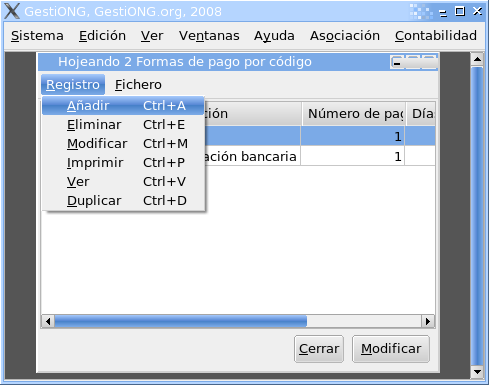
\includegraphics[width=6.332cm,height=5.186cm]{manual-img12.png}
\captionof{figure}[Hojeando formas de pago]{Hojeando formas de pago}
Utilizar el ratón para seleccionar menús, hacer click sobre botones,
ir al siguiente campo, etc. es intuitivo pero lento. La mayoría de
las operaciones tienen uno o varios equivalentes con el teclado. Por
ejemplo, los menús y los botones tienen generalmente una letra
subrayada: se pueden activar pulsando a la vez la tecla \textbf{Alt} y
esa letra subrayada. Por ejemplo, los botones Cerrar (Alt+C) y
Modificar (Alt+M) y los menús de la ventana principal: Sistema
(Alt+S), Ventanas (Alt+N), Asociación (Alt+O), etc.

Cuando un menú se despliega, algunas de sus opciones muestran a la
derecha del nombre una combinación de la tecla \textbf{Ctrl} y una
letra. Pulsar esa combinación de teclas elige esta opción del
menú aunque no esté visible. Por eso, cuando anteriormente pulsabas
\textbf{Ctrl+A} para añadir un registro, en realidad estabas
eligiendo el menú \textstyleGUIELEMENTREDUCED{Registro $\rightarrow $
Añadir}.

Por lo tanto, para añadir una nueva forma de pago utilizando solo el
teclado, pulsa \textbf{Alt+C} (Contabilidad), luego dad al cursor hacia
abajo varias veces hasta llegar a \textbf{Formas de pago...} y entonces
pulsa \textbf{Intro,} tras lo cual aparece la ventana de formas de pago
donde podrás pulsar \textbf{Ctrl+A} o bien \textbf{Alt+R} (Registro)
y luego \textbf{Intro}.
\end{minipage}
\end{center}


\begin{center}
\begin{minipage}{16.794cm}
{\centering\bfseries\itshape
Trucos para ir más rápidas (continuación)
\par}

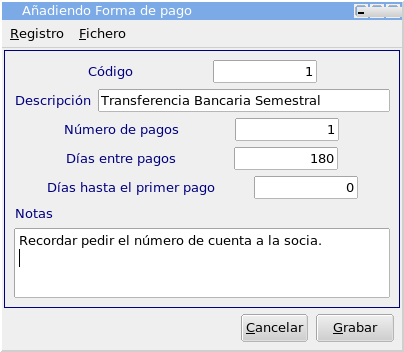
\includegraphics[width=5.877cm,height=5.225cm]{manual-img13.png}
\captionof{figure}[Añadiendo forma de pago]{Añadiendo forma de pago}
Una vez en el formulario para dar de alta la forma de pago, hay unos
recuadros para introducir la información sobre la nueva forma de
pago. Estos recuadros se llaman \textit{campos}. El cursor (indicador
parpadeante de la posición en la que estás tecleando) está ahora
en el campo \textstyleGUIELEMENTREDUCED{Notas}, que puede contener un
texto ilimitado, dividido quizás en párrafos.

Para avanzar al siguiente campo, puedes pulsar la tecla \textbf{Tab}
(tabulador, que se encuentra a la izquierda de la letra \textbf{Q}) o
bien la tecla \textbf{Intro} o bien la tecla \textbf{cursor abajo.}
Para volver al campo anterior, puedes pulsar la tecla \textbf{cursor
arriba} o bien \textbf{Mayús+Tab}. Ten en cuenta que no podrás
salir del campo \textstyleGUIELEMENTREDUCED{Notas}\textit{ }pulsando
\textbf{Intro} porque eso añade una nueva línea: tienes que salir
con \textbf{cursor abajo}, \textbf{Tab} ó
\textbf{Mayús}+\textbf{Tab.}

Una vez introducidos todos los datos necesarios del formulario, puedes
pulsar \textbf{Alt+G }( ó \textbf{F12} )\textbf{ }para
\textstyleGUIELEMENTREDUCED{Grabar} o bien \textbf{Alt+C} ( o
\textbf{Escape} ) para \textstyleGUIELEMENTREDUCED{Cancelar} los datos.
En general, la tecla \textbf{F12} graba o acepta los datos en cualquier
formulario y la tecla \textbf{Escape} los cancela.
\end{minipage}
\end{center}
\subsection{Añadiendo la información del contacto de vuestra
asociación}
Selecciona el menú \textstyleGUIELEMENT{Asociación$\rightarrow
$Contactos...} y pulsa \textstyleGUIELEMENT{Ctrl+A} o el botón
\textstyleGUIELEMENT{Añadir} para introducir un nuevo contacto.
Rellena los datos de vuestra asociación y pulsa
\textstyleGUIELEMENT{Grabar} ó \textstyleGUIELEMENT{F12}. Lee el
recuadro a la derecha para entender por qué los contactos están en
un fichero aparte.

\begin{center}
\begin{minipage}{8.1cm}
{\centering\bfseries\itshape
\label{ref:elficherodecontactos}El fichero de contactos
\par}

La información de carácter personal (nombre, dirección,
teléfonos, email, etc. ) de las personas físicas o jurídicas con
las que trabaja \appname se recogen en un fichero llamado
{\textquotesingle}Contactos{\textquotesingle}. Este fichero se
relaciona, pues, con cualquier otro fichero que tenga datos personales.
Las ventajas de este diseño son varias: se pueden reutilizar los
contactos y se evita duplicarlos si tenemos una persona que es a la vez
una socia y una acreedora; toda la información de carácter personal
está recogida en un solo fichero, lo cual es útil para el
cumplimento de la LOPD; y si un dato personal cambia, solo hará falta
cambiarlo en un lugar.
\end{minipage}
\end{center}
Selecciona ahora el menú \textstyleGUIELEMENT{Asociación
$\rightarrow $ Asociación...} y pulsa el botón
\textstyleGUIELEMENT{Contactos}. Aparece el formulario
{\textquotedblleft}\textbf{\textit{Eligiendo contactos por
CIF{\textquotedblright}}}. Selecciona el contacto que acabas de dar de
alta y pulsa \textstyleGUIELEMENT{Intro.} El \textstyleGUIELEMENT{CIF}
y el \textstyleGUIELEMENT{Nombre} del contacto aparecen en el
formulario de datos de la asociación. Graba.

\subsection{Añadiendo las personas socias }
Una vez grabados todos los datos anteriores, ya puedes comenzar a
añadir miembros a vuestro proyecto, es decir, las socias y socios de
vuestra asociación. Ve a
\textstyleGUIELEMENT{As}\textstyleGUIELEMENT{o}\textstyleGUIELEMENT{ciación$\rightarrow
$Proyectos...}, selecciona el primer proyecto y pulsa el botón
\textstyleGUIELEMENT{M}\textstyleGUIELEMENT{odificar} (o
\textstyleGUIELEMENT{Ctrl+M}). Ahora haz click sobre la pestaña
\textstyleGUIELEMENT{M}\textstyleGUIELEMENT{iembros} (o pulsa
\textstyleGUIELEMENT{Alt+M})\textbf{,} que contiene la lista de
miembros vacía. Pulsa \textstyleGUIELEMENT{Ctrl+A} y aparecerá el
formulario para añadir un nuevo miembro al proyecto.

Fíjate en los títulos de los formularios o ventanas: el que está
activo siempre tiene el fondo azul, en este caso
{\textquotesingle}\textbf{Añadiendo Miembro del
proyecto}{\textquotesingle}. El título ofrece siempre información
valiosa sobre el contenido de la ventana y lo que se está realizando,
por ejemplo, el formulario que está por detrás tiene por título
{\textquotesingle}\textbf{Modificando Proyecto: (id=1), 1, Socias y
socios ...}{\textquotesingle} y está con fondo negro porque su
ventana no está activa en este momento. 

Ahora vas a profundizar un poco más en el proceso de introducción de
datos en \appname tomando como ejemplo el formulario para añadir un
nuevo miembro al proyecto.

El primer campo, \textstyleGUIELEMENT{Proyecto}, está desactivado
porque no se puede cambiar y de ahí su fondo gris. El siguiente
campo, \textstyleGUIELEMENT{N{\textordmasculine} de soci@}, contiene ya
un valor sugerido: el siguiente número de socia disponible. El
siguiente es el \textstyleGUIELEMENT{Contacto}, donde además de poder
introducir un NIF/CIF y/o un nombre, se puede pulsar el botón
\textstyleGUIELEMENT{Contacto} con el ratón ( o
\textstyleGUIELEMENT{F3} ) para buscar el contacto.

\begin{center}
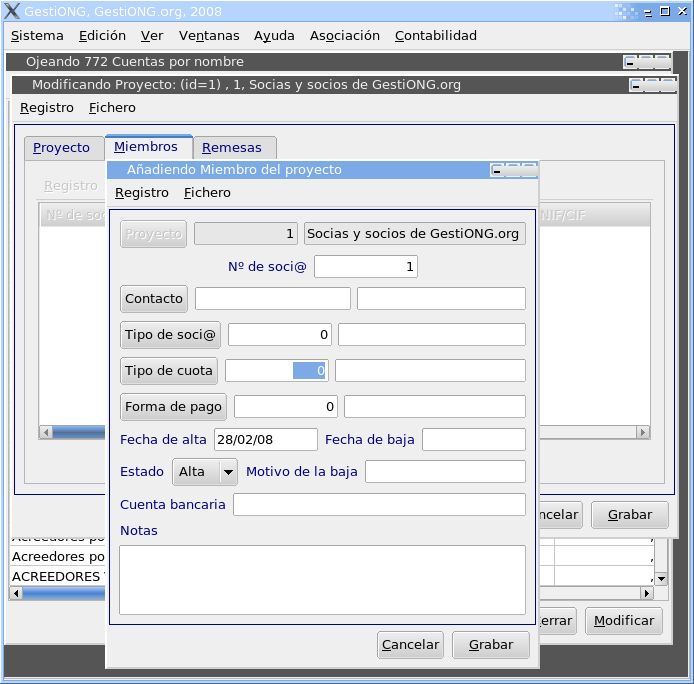
\includegraphics[width=8.772cm,height=8.823cm]{manual-img14.png}
\captionof{figure}[Añadiendo miembro del proyecto]{Añadiendo miembro
del proyecto}

\end{center}
Haz click en el botón \textstyleGUIELEMENT{Contacto} y aparecerá la
ventana del fichero de contactos. Si el que buscas ya estuviera dado de
alta, selecciónalo y pulsa el botón \textstyleGUIELEMENT{Elegir,}
si no, pulsa \textstyleGUIELEMENT{Ctrl+A} para añadir los datos del
contacto correspondiente a la socia o socio número 1. Cuando hayas
rellenado todos los campos, grábalo (botón
\textstyleGUIELEMENT{Grabar}) y elígelo (botón
\textstyleGUIELEMENT{Elegir}). Volverás al formulario de partida con
la información sobre el contacto rellena.

Ahora le toca el turno al \textstyleGUIELEMENT{Tipo de soci@}. Haz click
sobre el botón \textstyleGUIELEMENT{Tipo de soci@} y elige el tipo
apropiado pulsando el botón \textstyleGUIELEMENT{Elegir }o haciendo
\textstyleGUIELEMENT{doble-click} sobre él. Haz lo propio con el
\textstyleGUIELEMENT{Tipo de cuota}. Date cuenta de que cuando estás
eligiendo un contacto, un tipo de soci@ o cualquier otro registro,
puedes igualmente dar de alta nuevos registros pulsando
\textstyleGUIELEMENT{Ctrl+}A o modificarlos pulsando
\textstyleGUIELEMENT{Ctrl+M}.

Pero no siempre es necesario pulsar el botón para elegir un dato. Por
ejemplo, para elegir la forma de pago, puedes teclear un 1 en el
recuadro a la derecha del botón \textstyleGUIELEMENT{Forma de pago},
que es el código, y al pulsar \textstyleGUIELEMENT{Intro},
aparecerá a su derecha la descripción. Igualmente, si escribes la
descripción, aparecerá a la izquierda el código. Puedes incluso
escribir una descripción incompleta, y si existe una forma de pago
que contenga esa descripción incompleta, \appname la encontrará y
la mostrará. Si hubiese más de una forma de pago coincidente,
tendrías la opción de elegir de entre ellas la que andas buscando.
Imagina lo útil que es esto para buscar un contacto del que, por
ejemplo, solo te acuerdas de un apellido.

Vuelve de nuevo al formulario {\textquotedblleft}\textbf{Añadiendo
miembro del proyecto}{\textquotedblright} y rellena los restantes
campos: \textstyleGUIELEMENT{Fecha de alta},
\textstyleGUIELEMENT{Estado}, \textstyleGUIELEMENT{Fecha de baja y}
\textstyleGUIELEMENT{Motivo de la baja} (en su caso),
\textstyleGUIELEMENT{Cuenta bancaria }para el pago de las cuotas, etc.
Graba. Aparece otra vez el mismo formulario en blanco para añadir
otro proyecto. Pulsa la tecla \textstyleGUIELEMENT{Escape} o el botón
\textstyleGUIELEMENT{C}\textstyleGUIELEMENT{ancelar}.

Este es el procedimiento manual para añadir socias a los proyectos,
pero ahora vas a ver cómo puedes importar (introducir
automáticamente) los datos de vuestra hoja de cálculo de socias.

\subsection{Importando masivamente datos de socias y socios}
\label{ref:Importandomasivamente}Si ya tienes los datos de vuestras
socias y socios en una hoja de cálculo (si los tienes en algún otro
tipo de base de datos siempre podrás exportarlos a una hoja de
cálculo o similar), \appname te permite importarlos siempre y cuando
los adaptes a la plantilla que \appname te proporciona.

Abre el fichero de socias y elige en el menú la opción 
\textstyleGUIELEMENT{Tabla->Importar}. Dale al botón 
\textstyleGUIELEMENT{Mostrar plantilla para importar} y aparecerá una ventana con 
la plantilla que necesitas para importar los datos y una breve descripción de cada
columna. Copia todo el texto bajo
\textit{Puedes copiar y pegar este texto directamente a una hoja de cálculo:} y pégalo
en una hoja de cálculo. Ahora ve rellenando esta plantilla con los datos que quieres 
importar, lo cual puedes hacer fácilmente copiando y pegando desde tu hoja de cálculo
original.

\textbf{IMPORTANTE}: \textbf{Realiza una copia de seguridad de tu hoja
original puesto que vas a modificarla sustancialmente.}

{\itshape
Atencion: El nombre del socio o socia en \appname se almacena en un solo
campo, por lo tanto, si como en este ejemplo, lo tienes separado en
nombre y apellidos, debes unir ambas columnas.}

\end{center}
Lo único que falta es corregir la información sobre los tipos de
cuotas, tipos de socias y formas de pago para que se asocien
correctamente a cada miembro. La columna \textbf{Cuota} de tu hoja
contendrá posiblemente el valor de la cuota en euros, pero debe contener el
código que le has dado en el fichero de tipos de cuota en \appname y
su título debe ser \textstyleUserEntry{TIPOCUOTA.CODIGO}. Búscalo y
corrige su valor para cada socia. Haz lo mismo con las columnas
\textstyleUserEntry{TIPOSOCIA.CODIGO}, cuyos valores serían los
códigos con los que habéis dado de alta los tipos de soci@ en
\appname; y con \textstyleUserEntry{FORMAPAGO.CODIGO} que contendrá los códigos de
las formas de pago. Añade todas las formas de pago, tipos de socia y
cuotas que no estén ya en \appname. 

Una vez adaptada y revisada tienes que guardar la hoja en algún sitio
donde la encuentres posteriormente, con un formato especial: CSV. Desde
\textbf{LibreOffice}, ve a \textstyleGUIELEMENT{Archivo$\rightarrow
$Guardar como...}\textbf{, }dale un nombre,\textbf{ }elige el
\textstyleGUIELEMENT{Filtro: Texto CSV} y pulsa
\textstyleGUIELEMENT{Aceptar}. En la ventana que aparece
posteriormente, elige estos valores:

\begin{center}
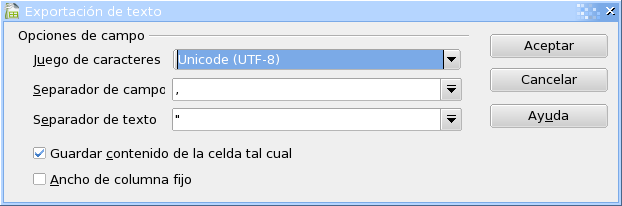
\includegraphics[width=12.748cm,height=4.309cm]{manual-img19.png}
\captionof{figure}[Opciones de exportación a CSV de
OpenOffice]{Opciones de exportación a CSV de OpenOffice}

\end{center}
y pulsa \textstyleGUIELEMENT{Aceptar}.

Ahora, de nuevo desde \appname, realiza primero la importación de los
contactos y luego la de las socias. Ve a
\textstyleGUIELEMENT{Asociación$\rightarrow $Contactos...}, elige la
opción \textstyleGUIELEMENT{Fichero$\rightarrow $Importar} y abre el
fichero CSV que acabas de guardar. \ Antes de comenzar con la
importación, se comprobará que los nombres de las columnas son
correctas y se avisará si has cometido algún error. Si todas las
columnas son correctas, irán apareciendo los contactos uno por uno de
forma que puedas corregir cualquier dato que esté incorrecto o
incompleto. Ve grabando uno por uno los contactos. Cuando hayas
finalizado, ve a \textstyleGUIELEMENT{Asociación$\rightarrow
$Proyectos...}, modifica el proyecto número \textit{1}, ve a la
pestaña de miembros (\textstyleGUIELEMENT{Alt+M}) y luego, bajo esa
pestaña, elige \textstyleGUIELEMENT{Fichero$\rightarrow $Importar...}
Abre el mismo fichero CSV y comenzará la importación de las socias.



\begin{center}
\begin{minipage}{15.189cm}
{\centering\bfseries\itshape
Resumen del proceso de importación de la hoja de socias
\par}

\liststyleLvi
\begin{enumerate}
\item \ Hoja: Poner títulos apropiados (nombre de los campos del
diccionario de datos) a las columnas \ (consultar los nombres en
\appname:\textstyleGUIELEMENTREDUCED{ Sistema$\rightarrow
$Configuración$\rightarrow $Diccionario de datos}).
\item \ \appname: Añadir los tipos de cuota, formas de pago y tipos de
socia que aparezcan en vuestra hoja y que no estén ya dados de alta.
\item \ Hoja: Asegurarse de que existen las columnas
\textstyleUserEntry{TIPOCUOTA.CODIGO, FORMAPAGO.CODIGO y
TIPOSOCIA.CODIGO}. Modificar sus valores para que coincidan con los
códigos en \appname.
\item \ Hoja: Añadir cualquier otro dato relevante sobre las socias,
como la cuenta bancaria, las observaciones, la nacionalidad, los
teléfonos, etc., con su título correspondiente.
\item \ Hoja: Exportarla a un fichero de texto con formato CSV.
\item \ \appname: Importar el fichero CSV desde el fichero de Contactos.
\item \ \appname: Importar el fichero CSV desde la pestaña de
\textstyleGUIELEMENTREDUCED{Miembros del proyecto} del fichero de
proyectos.
\end{enumerate}
\end{minipage}
\end{center}
